\documentclass{article}
\usepackage{amsmath}
\usepackage{amssymb}
\usepackage{enumerate}
\usepackage{graphicx}
\usepackage{float}

\begin{document}
\overfullrule=0pt
\def\frac#1#2{#1\over #2}
%
\def\bmatrix#1{\left[ \matrix{#1} \right]}
\def\be{{\beta}}
\def\toone{{t+1}}

%\def\frac#1#2{#1\over #2}
%\magnification=1200
\overfullrule=0pt

\noindent Macro Dynamics \hfill NYUAD \\
Fall 2, 2018 \hfill Thomas Sargent 
\vspace{.3cm}

\centerline{\bf Final Examination}
%\centerline{\bf Homework 3}


\medskip

\noindent{\bf Instructions:}  This is a take home exam.  100 points are possible. Points attached to each problem are stated
at the beginning of each problem. The exam is to be handed in on or before December 14.  
You are free to consult class notes and readings and also to discuss the questions with
other members of our class. Please hand in your own work.

\medskip

\noindent 
 

\medskip
\noindent{\bf Problem 1 \quad 10 points}

\medskip 

\noindent  Consider a consumer who wants to choose $\{c_t\}_{t=0}^T$ to maximize
\begin{align*}\sum_{t=0}^T \beta^tc_t  \quad  , \;\;  0< \beta<1\end{align*}
subject to the intertemporal budget constraint
\begin{align*} 
\sum_{t=0}^T R^{-t}[c_t-y_t]=0  \quad  ,   R>1 
\end{align*} where $c_t\geq0$ and $y_t>0$ for $t=0,\cdots,T$. Here $R>1$ is the gross interest rate $(1+r),\ \  r>0$. Assume $R$ is constant. Here $\{y_t\}_{t=0}^T $ is an exogenous sequence of ``labor income''.
\begin{enumerate}[\bf a.]
\item Assume that $\beta R < 1$. Find the optimal path $\{c_t\}_{t=0}^T$.
\item  Assume that $\beta R > 1$. Find the optimal path $\{c_t\}_{t=0}^T$.
\item Assume that $\beta R = 1$. Find the optimal path $\{c_t\}_{t=0}^T$.
\end{enumerate}
\medskip
\noindent{\bf Problem 2 \quad 20 points}

\medskip

\noindent
 A representative consumer has preferences ordered by
 $$ \sum_{t=0}^\infty \beta^t \ln (c_t), \;\;  0< \beta<1$$
 where $\beta = {\frac{1}{1+\rho}},\ \rho>0$, and $c_t$ is  consumption per worker.
The technology is $$ y_t=f(k_t)=zk_t^\alpha, \;\; 0<\alpha<1, \;\; z>0 $$
where $y_t$ is the output per unit labor and $k_t$ is capital per unit labor
\begin{align*}
y_t & =c_t+x_t+g_t \cr
  k_{t+1} & =(1-\delta)k_t+x_t, \;\;  0 < \delta<1 \cr
\end{align*}
and $x_t$ is  gross investment per unit of labor and $g_t$ is  government expenditures per unit of labor.
Assume a competitive equilibrium with a price system $\{q_t,\eta_t,w_t\}_{t=0}^\infty$ and a government policy $\{g_t,T_t\}_{t=0}^\infty$, where 
$g_t$ is government consumption and $T_t$ is a lump sum tax at time $t$.

 Assume that the government finances its expenditures by levying lump sum taxes. There are no distorting taxes. Assume that at time 0, the economy begins
 with a capital per unit of labor $k_0$ that equals the steady state value appropriate for an economy in which $g_t$ had been zero forever.
\begin{enumerate}[\bf a.]
	

\item 
Find a formula for the steady state capital stock when $g_t=0 \; \forall t$.
\item 
 Compare the steady state capital labor ratio $\overline{k}$ in the competitive equilibrium with the capital labor ratio $\tilde{k}$ that maximizes steady state consumption per capita, i.e ,
 $\tilde{k}$ solves $$\tilde{c}=\max_k \left( f(k)-\delta k \right) $$
Is $\tilde{k}$ greater than or less that $\overline{k}$? If they differ, please tell why. Is $\tilde{c}$ greater or less than $\overline{c} = f(\overline{k})-\delta  \overline{k}$? Explain why.
\item 
 Now assume that at time 0, $g_t$ suddenly jumps to the value $g={\frac{1}{2}}\overline{c}$ where
$\overline{c}$ is the value of consumption per capita in the initial steady state in which $g$ was zero forever. Starting from $k_0 = \overline{k}$ for the old $g=0$ steady state, find the time paths of $\{c_t,k_{t+1}\}_{t=0}^\infty$ associated with the new path $g_t=g>0 \; \forall t$ for government expenditures per capita.
Also show the time path for $\bar R_{t+1} \equiv (1-\delta) + f'(k_{t+1})$
Explain why the new paths are as they are.
\end{enumerate}

\medskip
\noindent{\bf Problem 3 \quad 10 points}

\medskip
\noindent
 A representative consumer has preferences ordered by
 $$ \sum_{t=0}^\infty \beta^t \ln (c_t), \;\;  0< \beta<1$$
 where $\beta = {\frac{1}{1+\rho}}, \rho>0$, and $c_t$ is the consumption per worker.
The technology is $$ y_t=f(k_t)=zk_t^\alpha, \;\; 0<\alpha<1, \;\; z>0 $$
where $y_t$ is the output per unit labor and $k_t$ is capital per unit labor
\begin{align*}
y_t & =c_t+x_t+g_t \\
  k_{t+1} & =(1-\delta)k_t+x_t, \   0 < \delta<1
\end{align*}
and $x_t$ is  gross investment per unit of labor and $g_t$ is  government expenditures per unit of labor.
Assume a competitive equilibrium with a price system $\{q_t,\eta_t,w_t\}_{t=0}^\infty$ and a government policy $\{g_t,T_t\}_{t=0}^\infty$, where
$g_t$ is government consumption and $T_t$ is a lump sum tax at time $t$.

 
Suppose that you observe the path for consumption per capita in figure 1. Say what you can about the likely behavior over time of $k_t$, $\bar R_t =[1 + (f'(k_t)-\delta)]$, $g_t$ and $T_t$. (You are free to make up any story that is consistent with the model.)

\medskip


\begin{figure}[H]
\label{figure_7_1}
\center
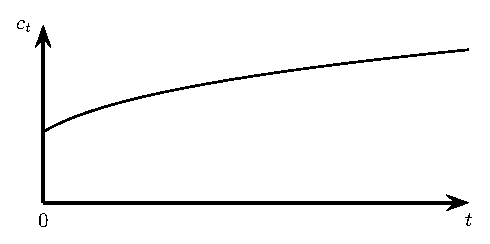
\includegraphics[width=2.5in]{fig_7_1.eps}
\caption{Consumption per capita.}
%\infiglist{fig_7_1}
\end{figure}




\medskip
\noindent{\bf Problem 4 \quad 10 points}

\medskip

\noindent Assume the same economic environment as in the previous  problem. Assume that someone has observed the  time path for $c_t$ in figure 2.
\medskip
\begin{figure}[H]
\label{fig_7_2}
\center
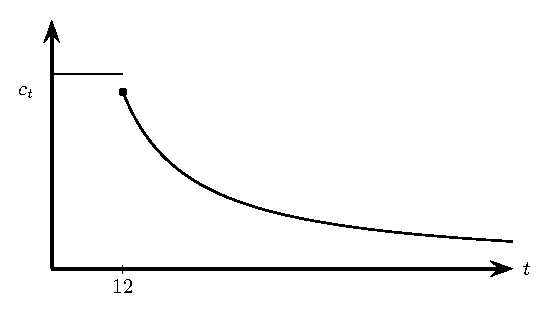
\includegraphics[width=2.5in]{fig_7_2.eps}
\caption{Consumption per capita.}
%\infiglist{fig_7_2}
\end{figure}
\begin{enumerate}[\bf a.]
	

\item Describe a consistent set of assumptions about the fiscal policy that explains this time path for
$c_t$. In doing so, please distinguish carefully between changes in taxes and expenditures that are \underbar{foreseen} versus \underbar{unforeseen}.

\item Describe what is happening to $k_t,\bar R_t$ and $g_t$ over time. Make whatever assumptions you must to get a complete but consistent story - here ``consistent'' means ``consistent with the economic environment we have assumed''.

\begin{figure}[H]
\label{FN_2}
\center
%\centerline{\epsfxsize=2.25truein\epsffile{FN_2_tom.eps}}
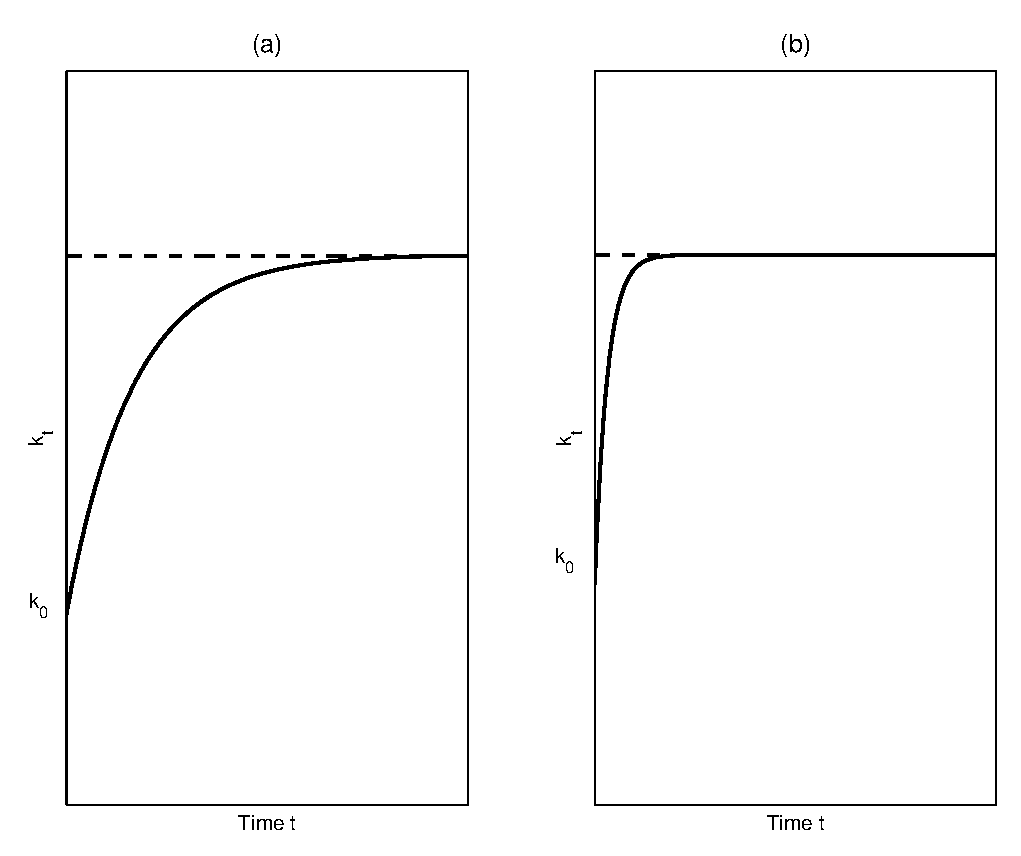
\includegraphics[width=2.25in]{fig_11_4.eps}
\caption{Capital stock as function of time in two economies with different values of $\gamma$.}
%\infiglist{FN_2}
\end{figure}

\end{enumerate}
\noindent{\bf Problem 5 \quad 10 points}

\medskip

\noindent
 The structure of the  economy is identical to that described 
 in the previous exercise.
Assume that $\{g_t, T_t\}_{t=0}^\infty $ are all constant sequences (their values don't change over time).
In this problem, we ask you to infer  differences
across two economies in which all aspects of the economy are identical {\it except} the parameter $\gamma$ in the utility function and maybe the level
of lump sum taxes $T_t$ imposed.  In both economies, $\gamma > 0$.  In one economy, $\gamma >0$ is high and in the other it is low.
Among other identical features, the two economies have identical government policies and identical initial capital stocks.\medskip
\medskip

\noindent{\bf a.}   Please look at figure 3. Please tell which outcome for $\{k_{t+1}\}_{t=0}^\infty$ describes the low $\gamma$ economy, and which describes the high $\gamma$ economy.
Please explain your reasoning.\medskip

\noindent{\bf b.}   Please look at figure 4. Please tell which outcome for $\{f'(k_t)\}_{t=0}^\infty$ describes the low $\gamma$ economy, and which describes the high $\gamma$ economy.
Please explain your reasoning.
\medskip

\noindent{\bf c.} Please plot time paths of consumption for the low $\gamma$ and the high $\gamma$ economies.



\begin{figure}[H]
\label{FN_3}
\center
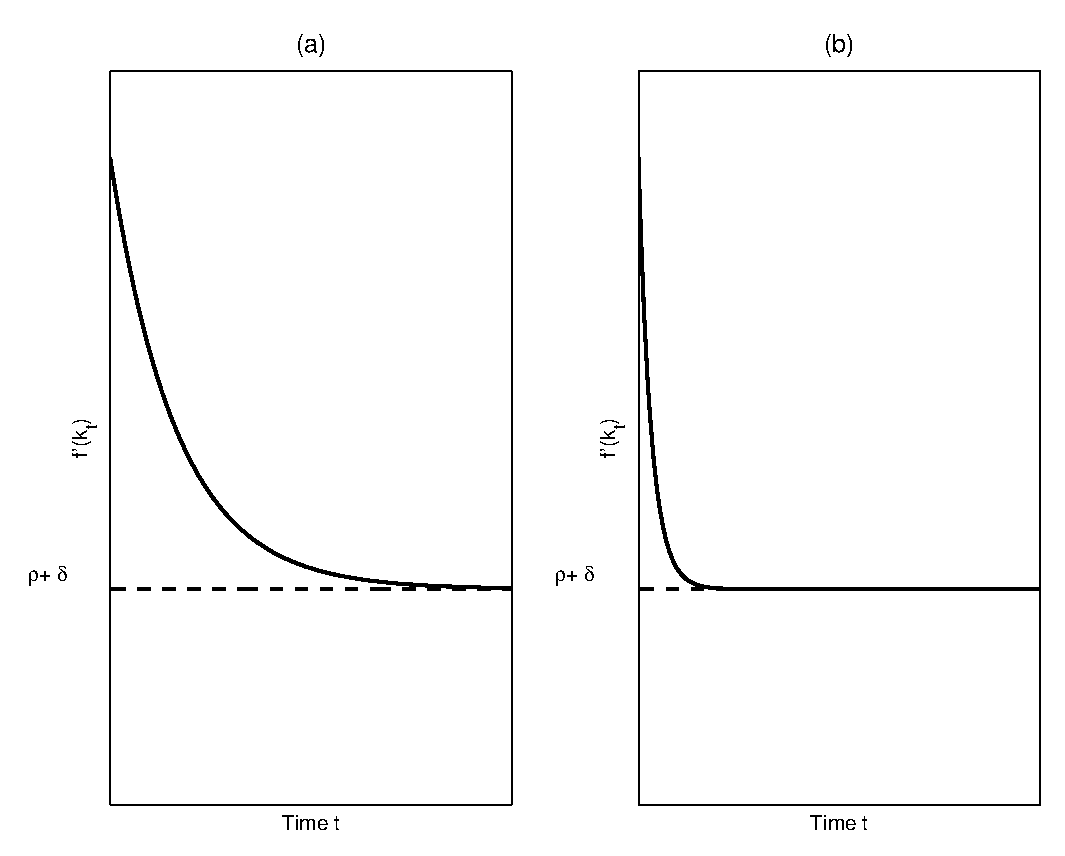
\includegraphics[width=2.25in]{fig_11_5.eps}
\caption{Marginal product of capital as function of time in two economies with different values of $\gamma$.}
\end{figure}

\noindent{\bf Problem 6 \quad 40 points} 

 \medskip
\noindent
{\bf Part  I}
\medskip 

\noindent
Consider the problem of a planner in a small economy. When the economy is closed to international trade, the planner chooses $\{c_t,k_{t+1}\}_{t=0}^\infty$ to maximize
$$ \sum_{t=0}^\infty \beta^t u(c_t), $$
where $ 0< \beta<1, \beta = {\frac{1}{1+\rho}}, \rho>0$
subject to
$$c_t+k_{t+1}=f(k_t)+(1-\delta)k_t,  \quad  \delta \in (0,1)$$
\noindent where $u(c_t)={\frac{c_t^{1-\gamma}}{1-\gamma}}$, $\gamma>0$, $f(k_t)=zk_t^\alpha$, and $0<\alpha<1$.


\medskip
\noindent
Let $\overline{k}$ be the steady state value of $k_t$ under the optimal plan.
\begin{enumerate}[\bf a.]
\item  Find a formula for $\overline{k}$.

\item Assume that $k_0<\overline{k}$. Describe time paths for $\{c_t,k_{t+1}\}_{t=0}^\infty$ and $\bar R_{t+1}=(1-\delta) + f'(k_{t+1})$.
\item What is the steady state value of $\bar R_{t+1}$?\medskip

\item Is $\bar R_{t+1}$ less or greater than its steady state value when $k_{t+1} < \overline{k}$?
\end{enumerate}

\medskip

\noindent {\bf Part  II}

\medskip 

\noindent
Now assume that the economy is open to international trade in capital and financial assets. Assume that there is a fixed world gross rate of return $R=\beta^{-1}$ at which the planner can borrow or lend, what is often called a `small open economy' assumption.
The planner can use the proceeds of borrowing to purchase goods on the international market. These goods can be used to augment capital or to consume.\medskip 

\noindent
Let $\overline{k}_0$ be the level of initial capital 
$(\overline{k}_0<\overline{k})$ before the country opens up to trade just before time 0.  Let $\overline{k}_0$ be the same initial capital per capita $\overline{k}_0 < \overline{k}$ studied in parts {\bf a}-{\bf d}.

\medskip

 \noindent
At time $t=-1$, after $\overline{k}_0$ was set, trade opens up. 
At time $t=-1$, the planner can issue IOU's or bonds in amount $B_{-1}$ and use the proceeds to purchase capital, thereby setting
$$k_0=\overline{k}_0+B_{-1} $$
where $B_{-1}$ is denominated in time -1 consumption goods. The bonds are one period in duration and bear the constant world gross interest rate $R=\beta^{-1}$.
For $t\geq 0$, the planner faces the constraints
$$ c_t+k_{t+1}+RB_{t-1}=f(k_t)+(1-\delta)k_t+B_t$$
Here $RB_{t-1}$ is the sum of interest and  principal on the bonds issued at $t-1$ and $B_t$ is the amount of one-period bonds issued at $t$. 

\medskip 

\noindent
The planning problem in the small open economy is now to choose $\{c_t,k_{t},B_t\}_{t=0}^\infty$ and $B_{-1}$, subject to $\overline{k}_0$ given. (Notice that $k_0$ is a choice variable and that $\overline{k}_0$ is an initial condition.)
Please solve the  planning problem in the small open economy and compare outcomes to those in the closed economy.
 Is  welfare $\sum_{t=0}^\infty \beta^t u(c_t)$ higher in the ``open'' or ``closed'' economy?






\end{document}

